\chapter{Estado del Arte}

% Una introducción al estrés...
El estrés ha sido considerado una problemática crítica y creciente en la sociedad moderna, afectando profundamente el 
bienestar mental y físico de las personas debido al ritmo de vida acelerado, las altas exigencias académicas y laborales, 
y la constante hiperconectividad \cite{mouadili2025advancing}. Como un mecanismo natural de supervivencia, el estrés activa 
el sistema nervioso autónomo (ANS), alterando el equilibrio entre el sistema nervioso simpático (SNS) y el sistema nervioso 
parasimpático (PNS) \cite{fontes2024enhancing, tao2025emotion_facial}. Sin embargo, la exposición crónica o excesiva a estas
 condiciones sin una regulación adecuada no solo reduce drásticamente la productividad, la concentración y la toma de 
 decisiones, tal como se evidencia en \cite{chatzaki2025overview, mouadili2025advancing}, sino que conduce a una 
 desregulación prolongada del eje hipotálamo-hipofisario-adrenal \cite{chatzaki2025overview}.
La literatura médica y psicológica advierte que esta hiperactivación constante es un desencadenante principal para el 
desarrollo de trastornos graves de salud mental, como ansiedad generalizada y depresión, además de diversos problemas 
físicos y fisiológicos \cite{chatzaki2025overview, mouadili2025advancing, singh2023stress_multi}. A nivel físico, el estrés 
crónico aumenta el riesgo de disfunciones cardiovasculares, hipertensión y debilitamiento del sistema inmunológico, e 
incluso se han documentado alteraciones estructurales en áreas del cerebro como la amígdala y la corteza prefrontal 
\cite{chatzaki2025overview, fontes2024enhancing, mouadili2025advancing, khomidov2024realtime}.

Debido a estas repercusiones sistémicas, investigaciones epidemiológicas han registrado un aumento global alarmante en su 
prevalencia, especialmente tras la pandemia de COVID-19, convirtiendo el monitoreo y gestión del estrés en una prioridad 
para la salud pública y ocupacional \cite{chatzaki2025overview}. Tradicionalmente, la cuantificación del estrés ha dependido 
de herramientas de autoinforme que requiere una participación consciente del individuo o por recomendación de un tercero, tales como cuestionarios estandarizados 
(por ejemplo, el STAI y el PSS) \cite{fontes2024enhancing, morales2022towards}. Si bien estos instrumentos gozan de validez 
clínica, presentan limitaciones operativas: son susceptibles al sesgo subjetivo y no permiten una evaluación continua en 
tiempo real, una brecha señalada por diversos autores en \cite{chatzaki2025overview, fontes2024enhancing, bahameish2024strategies}.

Para superar las barreras de la subjetividad bajo un enfoque positivista, la computación afectiva se ha volcado hacia la medición 
objetiva utilizando datos fisiológicos. Entre las diversas métricas corporales, la Variabilidad de la Frecuencia Cardíaca (HRV) se 
establece como el biomarcador más robusto y fiable para monitorear las respuestas de estrés \cite{fontes2024enhancing, bahameish2024strategies, brown2026remote}. 
Dado que la HRV refleja las variaciones de tiempo entre latidos cardíacos, actúa como una ventana directa a la actividad del ANS. En este contexto, 
situaciones de estrés provocan que la activación simpática suprima la actividad parasimpática, lo que deriva en una reducción medible de la 
variabilidad, mientras que en estados de relajación, la HRV aumenta \cite{brown2026remote}.

A pesar de la alta precisión de la HRV, su medición convencional requiere equipos de contacto que imponen restricciones en escenarios del 
mundo real: preparación lenta, dependencia de ambientes médicos y posibles irritaciones en la piel \cite{fontes2024enhancing, brown2026remote, yue2024facial_peak}. 
Es precisamente en este punto donde la necesidad de herramientas no invasivas ha impulsado la transición hacia la fotopletismografía remota (rPPG). 
Esta tecnología promete capturar las variaciones del volumen sanguíneo y la HRV utilizando únicamente cámaras estándar RGB sin contacto físico 
\cite{fontes2024enhancing, yue2024facial_peak}, abriendo la puerta a sistemas de diagnóstico escalables en entornos cotidianos, como aulas de clase o 
espacios de trabajo. \\*



% Saltando al rppg y la iluminación baja
La evolución de la fotopletismografía remota (rPPG) ha estado marcada por un debate constante sobre cuál es la representación matemática más robusta para 
extraer el pulso frente a las perturbaciones del entorno. Todo comenzó con W. Verkruysse principalmente y otros investigadores, considerados los pioneros absolutos de esta tecnología, quienes 
demostraron por primera vez que era posible medir el ritmo cardíaco utilizando cámaras comerciales y luz ambiental \cite{wu2026udarppg, yue2024facial_peak, cao2024stphys}. Ellos sentaron el estándar de la industria 
al descubrir que el canal verde (GREEN) de las cámaras captura la señal pulsátil más fuerte, debido a que la hemoglobina en la sangre absorbe la luz verde con 
mayor intensidad \cite{yang2022assessment_dl, wu2026udarppg}.

A partir de este hito fundacional, investigadores como M. Poh. y otros, que hacen parte del referente de trabajo base de \cite{transphys2023}, \cite{yue2024facial_peak}, \cite{wu2026udarppg},  intentaron limpiar el ruido ambiental del canal verde aplicando técnicas estadísticas de 
(Separación Ciega de Fuentes), específicamente el Análisis de Componentes Independientes (ICA). Es como M. Poh. en su enfoque pionero asumía que la señal del pulso y el ruido de la 
cámara eran fuentes completamente independientes que la matemática podía separar a ciegas, dicho de otra forma, propuso tratar el video como una mezcla de fuentes ruidosas y usar el ICA para desenredar 
el pulso cardiaco del ruido de la cámara, asumiendo que ambos son procesos que no se parecen en nada \cite{transphys2023}.

Aunque, en contraste con esta postura estadística, autores como De Haan y W. Wang criticaron la vulnerabilidad del método ICA ante los movimientos 
de la cabeza del sujeto según \cite{transphys2023, yue2024facial_peak}. Para solucionarlo, estos autores cambiaron el enfoque estadístico por modelos ópticos basados en la reflexión física de la luz sobre la 
piel, dando origen a los algoritmos tradicionales más famosos hoy en día: CHROM (de Chromatic model creado por De Haan) y POS (de Plane orthogonal to skin creado por W. Wang) \cite{yang2022assessment_dl, yue2024facial_peak, kim2022study}. Ellos demostraron que, al asumir un tono de piel estandarizado y proyectar 
los canales RGB en planos ortogonales, se podían eliminar los reflejos especulares causados por el sudor o el movimiento, logrando una señal mucho más limpia [\cite{transphys2023}, \cite{wu2026udarppg}, \cite{yue2024facial_peak}] .

En la literatura de la última década se mencionan a CHROM y POS, mas específico para (CHROM desde 2013 y POS desde 2017), como los métodos de procesamiento de señales más precisos, investigaciones muy recientes han 
comenzado a refutar la efectividad de estos cuando se introduce la variable más crítica: la baja iluminación. Autores como L. Xi. y W. Chen, entre otros, critican 
los fundamentos mismos de CHROM y POS en entornos oscuros. Argumentan que estos algoritmos asumen que la iluminación sobre la piel es constante; sin embargo, 
advierten que en la oscuridad, esta suposición colapsa por completo porque los canales de color rojo y azul pierden casi toda su información fisiológica y son 
devorados por el (ruido de cuantización) de la propia cámara, la cámara traduce la luz en números digitales. En la oscuridad, los cambios causados por el pulso 
son tan diminutos que la cámara no puede registrarlos con precisión y se ve obligada a redondear los valores. Ese error de redondeo genera una estática 
que es físicamente más fuerte que el latido del corazón, terminando por ocultarlo completamente \cite{yang2022image_en, yang2022assessment_dl, xi2022weighted}.

Curiosamente, y difiriendo de la creencia generalizada de que los modelos ópticos complejos siempre son superiores, estos autores demostraron de forma practica que 
en escenarios de iluminación críticamente baja, el método primitivo de Verkruysse (GREEN) y el estadístico (ICA) resultan ser más confiables que el avanzado 
algoritmo POS, el cual sufre una degradación extrema de su precisión al intentar mezclar canales de color vacíos \cite{yang2022image_en, yang2022assessment_dl, xi2022weighted}.\\

La siguiente tabla \ref{tab:algoritmos_tradicionales_rppg} contiene una breve descripción aprovechando los analísis de otros estudios:


\begin{table}[htbp]
    \centering
    \caption{Algoritmos tradicionales de extracción rPPG}
    \label{tab:algoritmos_tradicionales_rppg}
    \begin{tabular}{|p{2.5cm}|p{2.3cm}|p{3.2cm}|p{4.8cm}|}
        \hline
        \textbf{Algoritmo} & \textbf{Autor} & \textbf{Principio / Modelo Óptico}    & \textbf{Resumen del Objetivo y Mecanismo} \\ \hline
        GREEN              &  Verkruysse 2008   & Absorción espectral de la hemoglobina & Promedia espacialmente los píxeles del canal verde (G) en la región de interés (ROI) facial, aprovechando que esta longitud de onda presenta el mayor pico de absorción pulsátil de la sangre \cite{yang2022image_en, zhan2026hrv_long, debnath2026advanced_signal}  \\ \hline
        ICA / PCA Based    &  Lewandowska 2010  & Separación Ciega de Fuentes &  Descompone las trazas de 3 colores (RGB) en componentes estadísticamente independientes (ICA) o de máxima varianza (PCA) sin requerir enfoques ópticos \cite{yang2022image_en, transphys2023, debnath2026advanced_signal}  \\ \hline
        CHROM              &  Haan \& Jeanne 2013 & Diferencia de crominancia y Modelo Dicromático de Shafer & Proyecta el espacio RGB temporalmente normalizado en un subespacio de crominancia para eliminar los componentes de reflexión especular (brillo) \cite{nguyen2024artifact_resilience, debnath2026advanced_signal} \\ \hline
        PBV                &  Haan 2014         & Firma de Volumen Sanguíneo Pulsátil (Pulse Blood Volume) & Restringe las variaciones de color a una dirección conocida en el espacio RGB, definida por la firma espectral de absorción de la hemoglobina \cite{xu2023ivrrppg, liang2023selfadaptive} \\ \hline
        2SR                &  Wang 2015         & Spatial Subspace Rotation & Mide la rotación temporal del subespacio formado por los píxeles de la piel entre fotogramas consecutivos, no se centra o prioriza en el tono de la piel.  \cite{gupta2023privacy_pres, odinaev2024robust}   \\ \hline
        POS                &  Wang 2016         & Plane-Orthogonal-to-Skin  & Proyecta la señal RGB temporalmente normalizada en un plano ortogonal al vector de tono de piel para cancelar las variaciones de intensidad lumínica por movimiento. \cite{transphys2023, debnath2026advanced_signal, cho2025dualbranch, sabour2023ubfcphys}  \\ \hline
    \end{tabular}
\end{table}

\newpage

Con respecto al comportamiento de los algoritmos tradicionales frente a la iluminación deficiente, Green, al ser monocanal, evita la contaminación de otros canales 
ruidosos en baja iluminación, sin embargo, sufre una drástica caída de amplitud de señal y es extremadamente sensible al movimiento \cite{yang2022image_en}.
Según los resultados tiende a ser mas resistente que ICA y POS en cuanto a niveles de iluminación, pero en condiciones realistas los movimientos faciales son
propios y naturales. Según las pruebas de \cite{yang2022image_en}, en baja iluminación, los canales rojo (R) y azul (B) pierden la señal pulsátil y se 
llenan de ruido del sensor, rompiendo la independencia lineal y degradando la separación \cite{xi2022weighted}. En cuanto a POS, colapsa cuando la luz 
disminuye severamente, ya que el ruido de cuantización de la cámara pasa a dominar la proyección sobre el plano \cite{yang2022image_en, xi2022weighted}. PVB 
depende de un espectro de iluminación blanca constante, lo que significa que ante cambios bruscos de luz, la firma prestablecida deja de coincidir con el 
entorno según \cite{xu2023ivrrppg}. Según los experimentos de L. Xi y W. Chen, CHROM asume un tono de piel estandarizado y balance de blancos, cuando la 
luz cae y las lecturas RGB se acercan a cero, las relaciones de color se distorsionan ocasionando una degradación de la señal fotopletismografica \cite{yang2022image_en}.
Por último 2SR pierde precisión cuando la baja iluminación reduce el contraste del rostro, dificultando el seguimiento estable de las variaciones del 
ROI \cite{gupta2023privacy_pres, odinaev2024robust}.

En cuanto a la base de datos UBFC-Phys, en este estudio R. Sabour, Y. Benezeth y otros autores del estudio \cite{sabour2023ubfcphys}, mencionan que emplearon
eleccionaron POS debido a su eficiencia computacional y velocidad de ejecución para extraer la señal rPPG y posteriormente analizar la variabilidad del ritmo cardíaco.
Sin embargo como se ha mencionado anteriormente, POS resulta fuertemente afectado con el ruido de cuantización de la cámara dominando la proyección sobre el plano \cite{yang2022image_en, xi2022weighted}.

Frente a la dificultad de las fórmulas matemáticas estáticas para lidiar con el ruido en la oscuridad, se ha estado prestando mas atención hacia modelos y
arquitecturas basadas en datos, introduciendo las Redes Neuronales Convolucionales (CNN), como DeepPhys o PhysNet, capaces de aprender características espaciales 
de la piel directamente de los videos \cite{chen2024image_en, yang2022assessment_dl, nguyen2024artifact_resilience, xi2022weighted, effective2023cross,  dehnad2024factorize, zhuang2022fastbvp, speth2023hallucinated, xue2025noncontact, ma2025rfbayes, cen2025robust, liu2025synrppg}. 
Sin embargo, ante el continuo avance investigativo, la transición al Deep Learning tampoco está libre de críticas. Investigadores como Z. Yang. matizan el 
optimismo hacia las CNN, advirtiendo que estas redes sufren de un (sesgo inductivo local). Esto significa que las CNN se sobreajustan a las condiciones de 
iluminación ideales con las que fueron entrenadas en laboratorio y, en consecuencia, son menos precisas al intentar generalizar la extracción del pulso frente 
a variaciones lumínicas complejas o ruidos no vistos en el mundo real, esto es clave dado que podría parecer en muchos casos que tiene una clara ventaja frente a otros algoritmos \cite{yang2022assessment_dl}.

% %AgregadoSep2026
Aunque los Vision Transformers surgieron como la alternativa para superar la visión local de las CNN mediante mecanismos de auto-atención global, su 
aplicación pura en escenarios de baja iluminación presenta serias limitaciones. En primer lugar, los ViT carecen de sesgo inductivo espacial 
(\textit{spatial inductive bias}), lo que significa que no comprenden de manera intrínseca las relaciones de vecindad de los píxeles de la piel sin un 
volumen masivo de datos de entrenamiento \cite{transphys2023}. En condiciones de baja iluminación, donde la relación señal-ruido cae drásticamente 
debido a la escasez de iluminación, los mecanismos de atención global tienden a desestabilizarse, distribuyendo pesos de atención erróneos en regiones 
oscuras del fondo o ruido aleatorio del sensor en lugar de aislar la señal de rebote lúminica del rPPG.

Este debate en el estado del arte revela un vacío metodológico fundamental: la matemática óptica tradicional (como POS, CHROM y otros) falla en la oscuridad por la 
atenuación física de los colores, como mencionan en \cite{yang2022assessment_dl, yang2022image_en, xi2022weighted}.


A continuación se presenta una tabla \ref{tab:algoritmos_no_tradicionales_rppg} con una breve descripción de los algoritmos de aprendizaje profundo aplicados
a la extracción de señal fotopletismografica con los analísis extraidos de dichos estudios:

\begin{longtable}{|p{2.5cm}|p{2.3cm}|p{3.2cm}|p{4.8cm}|}
    \caption{Algoritmos de aprendizaje profundo para la extracción rPPG}
    \label{tab:algoritmos_no_tradicionales_rppg} \\
        \hline
        \textbf{Algoritmo}              & \textbf{Autor}              & \textbf{Naturaleza y Tipo de Arquitectura}                              & \textbf{Resumen del Objetivo y Mecanismo} \\ \hline
        DeepPhys                        &  Chen \& McDuff 2018        & CNN 2D Dual-Stream (Red convolucional de dos ramas)                     &  Separa la entrada en dos ramas: Apariencia, que extrae características de piel/ROI y genera máscaras de atención y Movimiento que calcula la diferencia normalizada entre tramas adyacentes. \cite{yang2022image_en, yu2023physformer}  \\ \hline
        PhysNet                         &  Yu et al 2019              & 3D-CNN Pura (Encoder-Decoder convolucional espacio-temporal)            &  Aplica convoluciones 3D directamente sobre secuencias de video (espacio y tiempo) para extraer la representación latente del pulso. \cite{yang2022image_en}  \\ \hline
        Self-Supervised RGB-NIR ViT     &  Park et al 2022            & Vision Transformer Multimodal de Fusión (RGB + Infrarrojo Cercano NIR)  &  Combina secuencias de video del espectro visible (RGB) e infrarrojo cercano (NIR) dentro de un tokenizador de video ViT con aprendizaje contrastivo auto-supervisado \cite{yu2024rgbnir}  \\ \hline
        EfficientPhys                   &  Liu et al. 2023            & Híbrido 2D-CNN + TSM + Swin Transformer / SASN                          &  Reemplaza las convoluciones 3D desplanzando canales a través del tiempo mediante el Temporal Shift Module (TSM) sobre capas 2D y aplicando atención Swin espacial \cite{dehnad2024factorize}  \\ \hline
        PhysFormer / PhysFormer++       &  Yu et al 2022/2023         & Híbrido 3D-CNN Stem + Tube Tokenizer + Temporal Difference Transformer  &  Extrae características locales con un Stem de 3D-CNNs, luego calcula atención global mediante Convoluciones de Diferencia Temporal (TDC) y usa una vía dual SlowFast \cite{yu2023physformer}  \\ \hline
        FactorizePhys                   &  Joshi. 2024                & Híbrido 3D-CNN + Factorized Self-Attention FSAM via NMF                 &  Utiliza Factorización de Matrices No Negativas (NMF) en el módulo FSAM sobre tensores 3D-CNN para calcular atención conjunta en espacio, tiempo y canales simultáneamente \cite{dehnad2024factorize}  \\ \hline
        ST-Phys                         &  Cao 2024                   & 3D-CNN con Convoluciones Dilatadas y Módulo de Realce                   &  Integra un Low-Light Enhancement Module (LEM), convoluciones dilatadas temporales (TDM) para ampliar el campo receptivo y atención espacial (SEM) \cite{cao2024stphys}. \\ \hline
        UDA-rPPG                        &  Wu 2024                    & Red con Anclaje de Dominio Geométrico-Fisiológico                       &  Utiliza un módulo GAEM para detectar y realzar el rostro en la oscuridad (anclaje geométrico), la red LS-Phys y la pérdida (Hp-loss) enfocada en picos espectrales \cite{wu2026udarppg}.  \\ \hline
        Phys-Vim / PhysMamba            &  Yan. 2024/Chang. 2025      & Modelo de Espacio de Estados (SSM / Vision Mamba)                       &  Sustituye la auto-atención cuadrática por un Escaneo Selectivo Multipat (MPSS) o dualidad estado-espacio (SSD), procesando videos largos a complejidad lineal $O(N)$ \cite{yan2025physmamba, chang2025physvim}.  \\ \hline
\end{longtable}

En la literatura reciente de rPPG, algunos algoritmos de aprendizaje profundo han sido evaluados o diseñados explícitamente para trabajar en entornos de 
baja iluminación o penumbra. Por un lado, arquitecturas como DeepPhys (2D-CNN dual), PhysNet (3D-CNN) y PhysFormer 
(basado en Transformers) fueron puestas a prueba en conjuntos de datos oscuros (como BH-rPPG y MMPD-rPPG) mediante la adición de un módulo de realce de 
imagen (IEM), el cual estandariza la iluminación previa a la extracción del pulso \cite{yang2022image_en}.

Por otro lado, se han desarrollado arquitecturas concebidas desde su origen para resistir la oscuridad extrema. Destaca ST-Phys, un marco convolucional 
3D no supervisado que integra un módulo de realce de baja luz (LEM) y convoluciones dilatadas temporales para procesar secuencias de video en niveles 
de iluminación de 1 a 100 lux \cite{cao2024stphys}. Del mismo modo, el modelo UDA-rPPG emplea una red espacio-temporal (LS-Phys) junto con un módulo de realce 
geométrico (GAEM) para asegurar la detección del rostro y extraer la señal rPPG en escenarios críticos de penumbra de entre 1.0 y 3.0 lux \cite{wu2026udarppg}.


A continuación se abordan los algoritmos de aprendizaje profundo para la extracción de rPPG y las métricas trabajadas en el desarrollo y evaluación de los
algoritmos:

\begin{table}[htbp] 
    \centering 
    \caption{Métricas de los algoritmos de aprendizaje profundo para la extracción rPPG} 
    \label{tab:metricas_algoritmos} 
    \begin{tabular}{|p{2.5cm}|p{2.3cm}|p{3.2cm}|p{4.8cm}|} 
        \hline 
        \textbf{Algoritmo} & \textbf{Métricas de evaluación} & \textbf{Resultados} & \textbf{Detalles de evaluación} \\ \hline
        % Juanda


        % Juanse
        PhysNet & \textbf{RMSE} y \textbf{R} (Correlación de Pearson) & RMSE: (1.812 BPM), R: 0.992 & Compararón contra métodos tradiconales como POS y CHROM \\ \hline
    \end{tabular}
\end{table}



% Hablando sobre los datasets y de donde suele salir la información para esto?

\newpage
\textbf{Validación y Bases de Datos: El Reto de la Calidad frente a la Corrección de Imagen}\\

En la siguiente tabla \ref{tab:bases_de_datos_video_rostro} se muestran las principales bases de datos de video mas usadas y empleadas por excelencia en la
mayoría de investigaciones relacionadas con extracción de señal fotopletismografica mencionadas en algunas investigaciones y sus detalles:

\begin{longtable}{|p{2.5cm}|p{2.3cm}|p{3.2cm}|p{4.8cm}|}
    \caption{Bases de datos utilizadas en investigaciones de extracción de señal rPPG}
    \label{tab:bases_de_datos_video_rostro} \\
        \hline
        \textbf{Base de Datos}      & \textbf{Autor}        & \textbf{Condicioones de iluminación}                                    & \textbf{Participantes, objetivo y sensores}  \\ \hline
        PURE                        &  Stricker. 2014       & Luz natural a través de ventana (con variaciones progresivas por nubes) & 10 sujetos (60 videos de 1 min a 30 fps) con sensor Oxímetro de pulso CMS50E (BVP y $SpO_2$ a 60 Hz) para medir la robustez de algoritmos rPPG ante movimientos de cabeza controlados. \cite{chang2025physvim, qiao2022revise} \\ \hline
        COHFACE                     &  Heusch. 2016         & Dos condiciones: iluminación natural e iluminación de estudio           & 40 sujetos (160 videos comprimidos en MPEG-4 a 20 fps). Oxímetro de pulso y cinturón respiratorio, creado para evaluar la extracción de rPPG en videos sometidos a alta compresión de video (256 Hz) \cite{zhan2026hrv_long,transphys2023} \\ \hline
        VIPL-HR                     &  VIPL-HR. 2018/2019   & Luz brillante, tenue/oscura y luz natural                               & 107 sujetos, 2,378 videos visibles (VIS) y 752 cerca del infrarrojo (NIR) con 3 cámaras. Oxímetro CONTEC CMS60C, para la evaluación no restringida de frecuencia cardíaca a gran escala integrando movimiento y variaciones de luz \cite{yang2022image_en, yu2024rgbnir} \\ \hline
        UBFC-rPPG                   &  Bobbia. 2019         & Luz artificial de estudio y luz ambiental de laboratorio                & 42 sujetos, 42 videos a 30 fps (640×480). Oxímetro de pulso transmisivo CMS50E (BVP) para evaluar la extracción de la señal rPPG y frecuencia cardíaca en un entorno estático de laboratorio con tareas matemáticas de tiempo \cite{yang2022image_en, yang2022assessment_dl, zhan2026hrv_long} \\ \hline
        BH-rPPG                     &  Yang. 2021           & 3 niveles de luz controlados: baja (8 lux), media (42.4 lux) y alta (104 lux) con luz no uniforme &  35 participantes, 105 videos (640×480 a 20–30 fps). Oxímetro de pulso CONTEC CMS50E para evaluar el impacto de variaciones severas de iluminancia sobre la estimación de rPPG \cite{yang2022image_en, yang2022assessment_dl}. \\ \hline
        UBFC-Phys                   &  Stricker. 2014       & Iluminación de laboratorio uniforme y constante                         & 56 sujetos con sensor Empatica E4 (BVP a 64 Hz, EDA, temperatura) y video 1024×1024 a 35 fps para estudiar las respuestas psicofisiológicas ante el estrés social mediante un protocolo TSST modificado (T1: reposo, T2: discurso, T3: aritmética) \cite{sabour2023ubfcphys} \\ \hline
        MMPD-rPPG                   &  Stricker. 2014       & 4 escenarios de luz: LED alta, LED baja, incandescente y luz natural    & 33 sujetos (fototipos Fitzpatrick 3–6), 660 videos (11 h) grabados con Samsung S22 Ultra. Oxímetro HKG-07C+ para probar la viabilidad de rPPG en teléfonos móviles bajo escenarios reales multidominio  \cite{yang2022image_en, cen2025robust} \\ \hline
        BUAA-MIHR / LRPD            &  Stricker. 2014       & Rango controlado de 1.0 a 35 lux en canales visible e Infrarrojo Cercano (NIR)  &  BUAA: 15 sujetos (165 videos en 11 niveles de lux). LRPD: 42 sujetos (168 videos en 3, 8 y 35 lux). Oxímetro de pulso de contacto para Analizar la estimación de rPPG en escenarios de extrema baja iluminación \cite{cao2024stphys, wu2026udarppg} \\ \hline
        CHILL                       &  Stricker. 2014       & Dos condiciones de estudio: Brillante (830 lux) y Oscura (14 lux)       & 45 participantes, 180 videos con ejercicios (flexiones de pecho/sentadillas) para elevar HR (54 a 141 bpm). Biosignalplux Explorer Kit (PPG a 1000 Hz) para investigar el impacto combinado de la baja iluminación y frecuencias cardíacas elevadas \cite{acharya2025reliability} \\ \hline
        
\end{longtable}


El rendimiento de los modelos y arquitecturas de Aprendizaje Profundo en la extracción rPPG depende de la naturaleza de los datos utilizados para 
su entrenamiento y validación. La literatura reciente evidencia una división en la elección de bases de datos (datasets): aquellas diseñadas para maximizar 
el ruido del mundo real y aquellas estructuradas para aislar variables fisiológicas puras.

Por un lado, investigadores como J. Tang y K. Chen introdujeron bases de datos altamente desafiantes como MMPD, la cual incluye 33 sujetos bajo cuatro 
condiciones de iluminación extremas, tonos de piel diversos y artefactos de movimiento severo, citados en los estudios de \cite{chen2024image_en, zhao2024masked}. De forma similar, 
G. Heusch y A. Anjos desarrollaron el dataset COHFACE, el cual introduce ruido adicional al estar severamente comprimido en formato MPEG-4 \cite{liu2025synrppg}. 
Si bien estos datasets son útiles para forzar a las redes neuronales a lidiar con escenarios incontrolados, presentan un problema metodológico para la 
investigación clínica: la saturación de variables (movimiento, compresión y luz simultáneamente) hace imposible cuantificar qué factor exacto está destruyendo 
la señal fisiológica.

Frente a la sobresaturación de ruido en bases como MMPD, investigadores enfocados en la fisiología pura han otorgado un valor grande a la familia de bases 
de datos UBFC (UBFC-rPPG y UBFC-Phys). T. Liu, en su estudio sobre generación de videos sintéticos, sostiene que UBFC-rPPG posee un valor superior como 
fuente de entrenamiento precisamente porque ofrece una calidad de video alta y carece de artefactos de movimiento u oclusión \cite{liu2025synrppg}. Al contar con un 
estándar de visual estático, bases como UBFC permiten a los investigadores aislar de manera precisa el impacto de una única variable (como la iluminación) 
sin los factores de confusión del movimiento facial \cite{liu2025synrppg}.
Aún más crítico para el contexto de esta investigación es el salto hacia el dominio psicológico. R. M. Sabour y Y. Benezeth desarrollaron UBFC-Phys, una base de 
datos diseñada explícitamente para estudios psicofisiológicos del estrés social \cite{sabour2023ubfcphys}. Y añadiendo el componente de computación afectiva a la ecuación, a diferencia de otros datasets que inducen emociones con simples videos, 
R. M. Sabour y Y. Benezeth estructuraron UBFC-Phys utilizando una versión modificada del Trier Social Stress Test (TSST), un protocolo clínico validado que incluye tareas de 
reposo, habla y aritmética mental, garantizando una inducción de estrés auténtica \cite{fontes2024enhancing, sabour2023ubfcphys}. Esta base de datos proporciona señales de Pulso de 
Volumen Sanguíneo (BVP) importantes para el calculo del HRV, y la Actividad Electrodérmica (EDA) sincronizadas con los videos, convirtiéndola en el entorno ideal para evaluar la clasificación del 
estrés una vez superado el reto de la extracción rPPG y clasificandolo como un recurso de caracter positivista al validar datos con sensores reales.\\

Al intentar resolver el desafío de la baja iluminación en las bases de datos, la comunidad científica se dividió en dos enfoques: alterar el video antes de que 
llegue a la red neuronal (pre-procesamiento) o robustecer la red neuronal misma.

Inicialmente, para el enfoque de pre-procesamiento, se intentó recurrir a métodos clásicos de visión computacional. Basándose en los fundamentos matemáticos 
establecidos por pioneros del procesamiento de imágenes como C. Poynton y T. Acharya, intentaron aplicar técnicas de aclarado fotograma por 
fotograma, como la Ecualización de Histograma (HE) y la Corrección Gamma (GC) \cite{chen2024image_en}. La lógica detrás de la Corrección Gamma dictaba que, al 
aplicar una transformación de potencia no lineal sobre los píxeles, se podía aumentar artificialmente el brillo y el contraste de los rostros en la sombra, 
haciendo que el algoritmo evaluara mejor la piel.

Sin embargo, esta práctica ha sido duramente refutada por la literatura reciente enfocada específicamente en rPPG. En su investigación, S. Chen. 
\cite{chen2024image_en} evaluaron estos filtros clásicos y demostraron que métodos como la Corrección Gamma y la Ecualización de Histograma logran que la imagen 
se vea mejor para el ojo humano, pero destruyen la consistencia temporal de la señal cardíaca. De forma paralela, L. Xi y W. Chen profundizaron en este problema, 
argumentando que la compensación de iluminación aplicada superficialmente rompe la coherencia de la variación de píxeles entre fotogramas sucesivos.

Dado que el rPPG no busca (imágenes estéticamente bonitas) sino variaciones micro-cromáticas perfectas a lo largo del tiempo, aplicar Corrección Gamma altera 
artificialmente la distribución del color tanto en la dimensión espacial como temporal \cite{yang2022assessment_dl}. 

Los resultados de S. Chen evidenciaron que aplicar estos filtros a videos 
en baja iluminación provocaba ganancias de Relación Señal-Ruido (SNR) negativas y causaba que arquitecturas neuronales, como DeepPhys y rPPGNet fallaran, elevando sus márgenes de error \cite{chen2024image_en}. 
En contraste con la idea de corrección Gama, investigadores como L. Xi coinciden en que es mucho más eficiente diseñar 
arquitecturas que aprendan características invariantes a la luz, en lugar de intentar arreglar los videos de prueba con filtros matemáticos estáticos que 
corrompen la señal fisiológica original se podría intentar realizar la operación inversa, es decir oscurecer los videos perfectos.


% Paso a comparación de algoritmos

La limitación de los métodos matemáticos tradicionales frente a los cambios ambientales impulsó una transición hacia arquitecturas basadas en datos (Deep Learning). 
En la tarea de extracción del pulso (regresión), la literatura ha demostrado que los algoritmos tradicionales presentan márgenes de error para 
entornos clínicos. Por ejemplo, estudios comparativos señalan que métodos analíticos como POS y CHROM exhiben una Tasa de Error Medio Porcentual (MER) del 9.85\% 
y 9.17\% respectivamente \cite{ma2025rfbayes}. Para superar esto, las Redes Neuronales Convolucionales (CNN) en dos y tres dimensiones lideraron los primeros avances. Arquitecturas 
como DeepPhys \cite{chen2024image_en}, basada en mecanismos de atención espacial y de movimiento, o modelos generativos como PulseGAN, lograron reducir drásticamente esta tasa de error 
porcentual (MER) a un notable 1.24\% bajo condiciones de laboratorio controladas \cite{ma2025rfbayes}.
Buscando superar el sesgo local de las convoluciones, se migró recientemente hacia la combinación de Redes neuronales convolucionales (CNN-3D) y los Vision Transformers (ViT). Z. Yu presentó PhysFormer, 
un modelo basado en auto-atención (self-attention) global que captura relaciones espacio-temporales de la señal a lo largo de todo el video \cite{yu2023physformer, yue2024facial_peak}. Esta arquitectura 
demostró una superioridad técnica en entornos bien iluminados. De hecho, algunas evaluaciones frente a variaciones de 
movimiento tienen como resultado que los ViT logran un Error Porcentual Absoluto Medio (MAPE) excepcionalmente bajo de 0.87\% (EfficientPhys) y 6.93\% (PhysFormer [Hibrido]), un resultado superior en comparación al 8.94\% 
obtenido por redes CNN 3D como PhysNet (Unicamente CNN-3D), valores tomados de \cite{dehnad2024factorize}.

El análisis profundo del estado del arte revela una desconexión metodológica: por un lado, se invierten esfuerzos en evaluar cómo la iluminación afecta el 
porcentaje de error (MAPE/MER) en la extracción de latidos, y por otro, se diseñan potentes clasificadores de estrés 
(superando el 90\% de exactitud y F1-Score) asumiendo que la señal de entrada siempre será ideal \cite{fontes2024enhancing}.
Sin embargo, no existe en la literatura actual un estudio que integre y cuantifique cómo la degradación lumínica impacta las métricas clínicas finales. 

La literatura explica una aparente superioridad de las CNN en escenarios ruidosos, la cual no se debe a una mejor capacidad de extracción fisiológica, sino a su 
(sesgo inductivo local), el cual actúa como un filtro natural contra la estática espacial de alta frecuencia generada por la oscuridad como explican Z. Chang y otros en \cite{chang2025physvim}. Los Vision Transformers, 
al carecer de este sesgo y depender de parches de atención global, requieren cantidades masivas de datos para aprender a ignorar el ruido de cuantización de la 
cámara \cite{chang2025physvim}. Cuando se enfrentan a luz deficiente sin un pre-procesamiento adecuado, la degradación espacial destruye los tensores de atención del ViT, elevando sus 
errores porcentuales a márgenes clínicamente inaceptables \cite{chang2025physvim}.\\

\textbf{Nuevas Fronteras: Datos Sintéticos y Modelos Mamba (SSM)}\\

Para resolver este estancamiento técnico, donde las CNN carecen de visión global y los ViT son computacionalmente frágiles ante el ruido lumínico, la 
investigación más reciente (2024-2025) ha propuesto dos grandes progresos.
El primero es la inyección de datos sintéticos mediante modelos generativos para robustecer el entrenamiento no supervisado. T. Liu propuso la arquitectura 
SAFNet (Syn-rPPG), demostrando que alimentar a los modelos con videos donde se ha transferido artificialmente oscuridad y artefactos de movimiento obliga a la 
red a volverse resistente al ruido. Con esta técnica de datos sintéticos, SAFNet logró un MAE sobresaliente de 0.17 bpm en la base de datos UBFC-rPPG \cite{liu2025synrppg}, superando 
incluso a los mejores enfoques supervisados.

El Segundo es el reemplazo total de los Transformers por los nuevos Modelos de Espacio de Estados (SSM), específicamente la arquitectura Mamba \cite{chang2025physvim, yan2025physmamba}. 
Z. Chang introdujo Phys-Vim, un modelo que logra capturar dependencias espacio-temporales a largo plazo pero con una complejidad computacional lineal, eliminando 
el prohibitivo costo de atención cuadrática de los ViT \cite{chang2025physvim}. Esto significa que el costo cuadrático de un ViT implica que a medida que aumenta la duración del 
video, el consumo de memoria y procesamiento de la red crece de forma exponencial (haciéndolos inviables para monitoreo en tiempo real), mientras que la 
complejidad lineal de la arquitectura Mamba permite que el esfuerzo computacional crezca solo de forma proporcional a la duración del video, logrando el mismo 
nivel de percepción global pero de manera sumamente ligera y rápida \cite{chang2025physvim}. En pruebas de validación cruzada (de UBFC-rPPG hacia PURE), Phys-Vim redujo el MAE en un 73.3\% frente a modelos Transformer previos como Spiking-PhysFormer, alcanzando un MAE de 0.72 bpm y un RMSE de 1.90 bpm, utilizando un 82\% menos de 
parámetros computacionales según los resultados consignados en \cite{chang2025physvim}.

De manera paralela, Z. Yan desarrolló PhysMamba, una arquitectura de vía dual que integra la dualidad de espacio de estados (SSD) con consultas de múltiples 
escalas (MQ) para intercambiar información en el dominio del tiempo y la frecuencia \cite{yan2025physmamba}. Al probarse en las condiciones de luz degradada y ruido de la base de datos 
MMPD, PhysMamba logró un MAE de 2.84 bpm y un RMSE de 6.41 bpm, superando ampliamente a modelos como TS-CAN (MAE de 8.97) y EfficientPhys (MAE de 12.79) \cite{yan2025physmamba}.

Esta revisión crítica evidencia que la ciencia continua descifrando cómo equilibrar la capacidad de modelado global de la IA con la resistencia 
física al ruido lumínico. Queda claro que evaluar un algoritmo rPPG en condiciones ideales de laboratorio no ofrece garantías sobre su aplicabilidad clínica.
La opciones alternativas comprenden entre trabajar modelos nuevos que puedan comprender mejor la degradación lumínica, profundizar mayormente el funcionamiento
de las arquitecturas tradicionales o implementar características que permitan converger en la mezcla de modelos y generar resultados adaptables.

% Final del texto del estado del arte
\textbf{Brecha de Investigación y Posicionamiento del Proyecto}\\

La revisión del Estado del Arte evidencia una convergencia clara de problemas metodológicos no resueltos:

\begin{enumerate}
    \item \textbf{Vulnerabilidades arquitectónicas contrastantes:} Las arquitecturas de aprendizaje profundo exhiben debilidades teóricas opuestas ante la falta 
    de luz. Mientras que los modelos avanzados como los Vision Transformers (ViT) corren el riesgo de amplificar el ruido espacial de la cámara al carecer de un 
    sesgo inductivo local, las Redes Neuronales Convolucionales (CNN) clásicas sufren de campos receptivos limitados que restringen su comprensión temporal a 
    largo plazo. El nivel exacto de resiliencia comparativa entre ambos enfoques bajo oscuridad pura sigue siendo una pregunta abierta en la literatura.

    \item \textbf{Limitaciones en el pre-procesamiento:} Los intentos de solucionar la oscuridad aplicando filtros tradicionales de visión computacional sobre la 
    imagen (como la Corrección Gamma) resultan clínicamente inviables, ya que destruyen la coherencia temporal de la señal y alteran las micro-variaciones 
    cromáticas del pulso cardíaco.

    \item \textbf{Sobresaturación en los Datasets:} Aunque existen bases de datos con iluminación variable en la literatura (como MMPD), la sobresaturación 
    simultánea de variables (movimiento severo, compresión de video y luz) hace imposible aislar y medir el efecto puro de la oscuridad.

    \item \textbf{Desconexión entre la extracción de la señal y la evaluación clínica del estrés:} Mientras que estudios recientes de visión computacional se 
    limitan a medir la degradación por iluminación en términos de error de estimación del pulso (MAE o RMSE) \cite{chen2024image_en, nguyen2024artifact_resilience}, las investigaciones enfocadas en la detección del 
    estrés asumen condiciones lumínicas ideales para extraer la Variabilidad de la Frecuencia Cardíaca (HRV) y lograr altas métricas de clasificación \cite{fontes2024enhancing, bahameish2024strategies}. Como 
    advierten J. P. Cobá Juárez Pegueros y J. Rodríguez-Arce \cite{rodriguez2025datasets}, existe una necesidad crítica de evaluar los modelos de estrés en escenarios no controlados para 
    garantizar su fiabilidad. Sin embargo, en la literatura actual no se ha cuantificado cómo el colapso inicial del rPPG frente a la oscuridad se propaga en 
    cascada hasta destruir la precisión del diagnóstico psicológico.

\end{enumerate}

%ModificadoSep2026
En consecuencia, el presente proyecto de investigación se posiciona como una propuesta 
metodológica para hacer frente a esta brecha en la literatura. Aprovechando el rigor 
clínico y la estabilidad del protocolo de estrés psicofisiológico (TSST) proporcionado 
por la base de datos UBFC-Phys, esta investigación evitará la alteración de los videos 
mediante algoritmos sintéticos de mejora visual que puedan introducir artefactos en la 
señal. En su lugar, se identificará y seleccionará, a partir de la evidencia reportada en 
la literatura, el modelo o combinación de arquitecturas con mayor resistencia intrínseca 
ante una degradación lumínica controlada, evaluando su desempeño en penumbra sin recurrir 
a correcciones visuales previas. De este modo, el objetivo final no se limita a medir el 
error en la estimación del pulso (mediante métricas de regresión como MAE y RMSE), sino a 
demostrar en qué medida la preservación de la señal fisiológica rPPG permite sostener la 
fiabilidad en la clasificación binaria del estrés, evaluando su impacto directo en métricas 
de diagnóstico clínico como Accuracy y F1-Score.




\section{Categorías de Análisis}

La literatura seleccionada fue agrupada en cuatro categorías de análisis que representan las dimensiones críticas del presente proyecto. Estas categorías 
permiten tener un enfoque de entender el estrés y como se puede medir, transitar desde la física del sensor clinico hasta los datasets usualmente validados con caracter positivista.

\subsection{Categoría 1: Principios Ópticos y Evolución Matemática en rPPG}
Esta categoría establece las bases biológicas y las limitaciones de los modelos de procesamiento tradicionales. Para este pilar, se integraron estudios 
fundamentales y de revisión sistemática \cite{yang2022assessment_dl, camerabased2024wang}, los cuales proporcionan la justificación sobre la interacción de la 
luz con la hemoglobina en el canal verde. Asimismo, se analizan los métodos de Separación Ciega de Fuentes y modelos ópticos de reflexión física 
\cite{transphys2023, yang2022assessment_dl, yue2024facial_peak}. Esta agrupación es indispensable porque demuestra teóricamente por qué los algoritmos clásicos 
como POS y CHROM colapsan ante la degradación lumínica.

\subsection{Categoría 2: Arquitecturas de Aprendizaje Profundo y Resiliencia Lumínica}
Aquí se evalúa la robustez computacional de la Inteligencia Artificial. Se seleccionaron las investigaciones sobre redes convolucionales (CNN), Vision 
Transformers (ViT), modelos hibridos y modelos de espacio de estados (Mamba) \cite{yu2023physformer, chang2025physvim, cen2025robust, yan2025physmamba}, ya que definen la 
frontera actual del rendimiento. Complementariamente, se incluyeron documentos que aportan información sobre (alucinaciones) de latidos, ataques de presentación, 
sistemas de privacidad y datos sintéticos \cite{wu2026udarppg, speth2023hallucinated, gupta2023privacy_pres, xu2023ivrrppg, qiao2022revise}. Este bloque 
fundamenta por qué se requiere someter a las redes a un oscurecimiento controlado.\\

La evaluación de la robustez de los modelos de Aprendizaje Profundo (Deep Learning) frente a la atenuación de la luz exige un marco experimental que aísle 
rigurosamente las variables bajo análisis. En el contexto de la computación afectiva, la base de datos UBFC-Phys
 se posiciona como el estándar de validación debido a su diseño metodológico positivista. A diferencia de otros conjuntos de datos enfocados en ruido 
 descontrolado o expresiones faciales simples, UBFC-Phys proporciona registros de video de alta calidad sincronizados con sensores de contacto clínicos 
 (como el dispositivo Empatica E4), capturando señales de Pulso de Volumen Sanguíneo (BVP) esenciales para el cálculo de la Variabilidad de la Frecuencia 
 Cardíaca (HRV) bajo un protocolo clínicamente validado de inducción de estrés (Trier Social Stress Test - TSST) \cite{debnath2026advanced_signal, cho2025dualbranch}. La ausencia de oclusiones y movimientos 
 severos en esta base de datos es clave, ya que permite aislar y cuantificar de manera pura el impacto de la 
degradación de la iluminación en la señal fisiológica, eliminando variables de confusión comunes en entornos incontrolados.\\

No obstante, dado que UBFC-Phys fue registrada bajo condiciones de iluminación ideales de laboratorio \cite{debnath2026advanced_signal}, la literatura científica menciona la alteración 
artificial de estos entornos para evaluar la robustez. La modificación de los fotogramas mediante técnicas de oscurecimiento digital y la 
inyección de artefactos visuales constituye un enfoque metodológico validado para probar modelos rPPG en escenarios desafiantes \cite{kim2022study}. Investigaciones lideradas 
por G. Cho y M. Kim \cite{cho2025dualbranch}. demuestran que el brillo de los fotogramas debe ser manipulado matemáticamente a través de transformaciones 
lumínicas en los pixeles del rosto, una técnica preferible sobre los filtros de realce de brillo tradicionales (como la corrección Gamma o ecualización) que corrompen la 
dimensión temporal del latido y la señal de espectro verde. Para simular fielmente las limitaciones de los sensores ópticos reales en condiciones ambientales oscuras, se requiere 
complementar la pérdida de brillo con la inyección de ruido de cuantización (ruido Gaussiano con media cero), permitiendo recrear la estática de alta 
frecuencia que físicamente enmascara las micro-variaciones cromáticas de la piel \cite{debnath2026advanced_signal}.

\subsection{Categoría 3: Computación Afectiva y Diagnóstico Clínico del Estrés}
Dado que la extracción del pulso es un medio para alcanzar una evaluación médica, esta categoría articula el video con la salud mental. Se seleccionaron 
trabajos que detallan cómo las métricas de HRV se transforman en diagnósticos de estrés, fatiga y emociones 
\cite{fontes2024enhancing, mouadili2025advancing, morales2022towards, bahameish2024strategies, kakhi2025fatigue_wear, hsu2025basic_emotion}. De igual forma, 
se integraron revisiones sobre conjuntos de datos abiertos \cite{chatzaki2025overview, rodriguez2025datasets, odinaev2024robust}, lo que permite plantear la 
hipótesis de que la degradación lumínica generará un error en cascada en el diagnóstico final.

\subsection{Categoría 4: Protocolos Clínicos, Bases de Datos y Métricas de Validación}
Para cuantificar el impacto de la oscuridad, se requiere un marco experimental estandarizado. Esta categoría agrupa los documentos que introducen y evalúan 
bases de datos clave como UBFC-Phys, MMPD, rPPG-10, CHILL y COHFACE 
\cite{acharya2025reliability, sabour2023ubfcphys, rodrigues2025evaluating, benezeth2024video, nguyen2024artifact_resilience, yang2022assessment_dl}. 
Finalmente, se incluyeron estudios sobre índices de calidad de la señal \cite{ma2025rfbayes, debnath2026advanced_signal}, estableciendo las métricas de 
regresión (MAE, RMSE) y clasificación (Accuracy, F1-Score) con las que se validará el desempeño del sistema.

\section{Criterios}
\subsection{Criterios de Inclusión}
\begin{itemize}
    \item \textbf{Rango Temporal:} El núcleo de la investigación se centra en documentos publicados entre enero de 2022 y abril de 2026. Se prioriza el periodo 
    2022-2024 para la evolución de modelos CNN y el periodo 2024-2026 para el estado del arte de Vision Transformers (ViT) y modelos emergentes. 
    Se incluyen excepcionalmente obras seminales previas a 2022 para establecer el fundamento histórico de la rPPG.
    \item \textbf{Tipo de Fuente:} Artículos de revistas indexadas, actas de conferencias (como IEEE/CVF, CVPR, NeurIPS) y revisiones sistemáticas de literatura.
    \item \textbf{Bases de Datos e Idioma:} El proceso de búsqueda se realizó principalmente a través del sistema de recursos digitales de la Universidad de 
    La Salle Colombia, en bases de datos de alto impacto como IEEE Xplore, ScienceDirect (Elsevier), PubMed y Scopus. Se empleó Google Scholar como herramienta 
    de rastreo complementaria y se consultaron repositorios de pre-publicación (\textit{arXiv}) para integrar avances de frontera correspondientes al año 2026. 
    Se seleccionaron exclusivamente documentos en inglés, dado que este constituye gran parte del estándar para definiciones de computación afectiva.
    \item \textbf{Temática:} Estudios que integren de forma explícita el uso de rPPG con la detección de estrés o fatiga, análisis de robustez ante 
    baja iluminación y comparativas de rendimiento entre arquitecturas de Deep Learning.
\end{itemize}
\subsection{Criterios de Exclusión}
\begin{itemize}
    \item \textbf{Sensores de contacto:} Se descartan investigaciones basadas exclusivamente en dispositivos físicos adheridos al cuerpo 
    (ECG, bandas de pecho, wearables) que no incluyan el uso de video o cámaras para la extracción de la señal.
    \item \textbf{Opacidad Técnica:} Quedan excluidos los artículos que reportan resultados de software comercial tipo caja negra, uso privativo, donde no se describe la 
    arquitectura del modelo (CNN, ViT, etc.) ni los detalles del entrenamiento.
    \item \textbf{Calidad de la Fuente:} No se incluyen publicaciones en blogs, sitios de noticias, artículos de opinión o documentos de conferencias que no 
    cuenten con un proceso comprobable de revisión por pares (No marcados con indicador \textit{peer-reviewed}).
    \item \textbf{Inconsistencia Temática:} Se excluyen estudios de visión artificial enfocados únicamente en biometría (identidad, género, edad) o 
    reconocimiento de expresiones faciales que no realicen extracción de pulso (HR/HRV) ni diagnóstico de estrés.
    \item \textbf{Restricción de Idioma:} Documentos publicados en idiomas distintos al inglés, con el fin de garantizar la precisión técnica de los términos y 
    métricas estándarizadas en la literatura global de Inteligencia Artificial, estudio del estrés, bases de datos fisiológicas y computación afectiva.
\end{itemize}

\section{Metodología de la revisión sistemática}

\subsection{PRISMA}
Bajo las directrices de la metodología PRISMA, se ejecutó un proceso de selección de artículos para consolidar la base bibliográfica de la investigación, 
utilizando ecuaciones de búsqueda diseñadas para cubrir el espectro técnico del proyecto. El acceso a la literatura se realizó principalmente a través del 
sistema de recursos digitales de la Universidad de La Salle, consultando bases de datos indexadas como IEEE Xplore, ScienceDirect (Elsevier), PubMed y Scopus, 
además del motor complementario Google Scholar y el repositorio técnico arXiv. La búsqueda se organizó en cuatro pilares fundamentales, seleccionando términos 
específicos que permitieran identificar tanto los fundamentos físicos como las innovaciones en IA y diagnóstico clínico:

\begin{itemize}
    \item \textbf{Pilar 1: Justificación del problema (El reto de la iluminación)} \\
    \textit{Justificación:} Estos términos se seleccionaron para localizar estudios que analizan el comportamiento de los sensores y el ruido de cuantización 
    cuando la señal lumínica es insuficiente para los métodos tradicionales.
    \begin{itemize}
        \item \textbf{Palabras clave:} \textit{Low-light rPPG, remote photoplethysmography, dark environment, darkness, low lux, illumination robustness, 
        image enhancement, quantization noise, signal-to-noise ratio, SNR in rPPG.}
    \end{itemize}

    \item \textbf{Pilar 2: Arquitecturas y Tecnologías de IA} \\
    \textit{Justificación:} Se utilizaron para identificar la evolución desde las redes clásicas hasta los modelos de atención global y espacio de estados, 
    permitiendo la comparación entre el sesgo inductivo local y la percepción global.
    \begin{itemize}
        \item \textbf{Palabras clave:} \textit{Deep Learning rPPG, remote photoplethysmography, CNN, ConvNet, Vision Transformers, ViT, PhysFormer, State Space Models, SSM, 
        spatio-temporal attention, contactless monitoring, global attention, self-attention mechanism}
    \end{itemize}

    \item \textbf{Pilar 3: Fisiología, Comprensión Clínica del Estrés y Salud Mental} \\
    \textit{Justificación:} Estos ítems permiten vincular la extracción técnica del pulso con la aplicación clínica, enfocándose en los biomarcadores que validan 
    el diagnóstico de estrés y fatiga cognitiva.
    \begin{itemize}
        \item \textbf{Palabras clave:} \textit{Stress detection, remote photoplethysmography, Heart Rate Variability, HRV, affective computing, mental health monitoring, anxiety recognition, 
        autonomic nervous system, ANS, cognitive load.}
    \end{itemize}

    \item \textbf{Pilar 4: Metodología, Datasets y Validación} \\
    \textit{Justificación:} Seleccionados para estándarizar la evaluación del proyecto mediante el uso de bases de datos públicas y métricas de error aceptadas 
    unánimemente por la comunidad científica.
    \begin{itemize}
        \item \textbf{Palabras clave:} \textit{UBFC, UBFC-Phys, PURE, MAHOB-HCI, MMPD dataset, rPPG benchmarking, Mean Absolute Error, MAE, RMSE, Pearson correlation, r, F1-Score.}
    \end{itemize}
\end{itemize}

Dichos términos se articularon mediante ecuaciones de búsqueda empleando operadores lógicos (AND, OR) y signos de agrupación (paréntesis). El diseño de estas 
cadenas de búsqueda contó con el apoyo de Inteligencia Artificial para optimizar la precisión de los resultados. Esta sintaxis permitió refinar el filtrado de 
información, asegurando que la recuperación de documentos fuera altamente pertinente para los objetivos específicos de la investigación.\\

El siguiente es un ejemplo de un prompt de búsqueda:
\begin{quote}
\centering
\textit{(''remote photoplethysmography'' OR ''rPPG'') AND (''stress detection'' OR ''anxiety recognition'') AND (''Heart Rate Variability'' OR ''HRV'' OR ''Autonomic Nervous System'')}
\end{quote}


\newpage
El flujo de selección se dividió en las siguientes fases de filtrado:

\begin{enumerate}
    \item \textbf{Identificación:} Se obtuvieron un total de \textbf{138 registros} a través del portal digital de la Universidad de La Salle y motores de búsqueda especializados.
    \item \textbf{Filtrado:} Tras eliminar 22 documentos duplicados y fuentes no indexadas, la muestra se redujo a \textbf{116 registros} para la revisión inicial de títulos y resúmenes.
    \item \textbf{Elegibilidad:} Se evaluaron \textbf{77 artículos} mediante lectura, descartando 39 documentos con metodologías opacas o falta de métricas comparativas.
    \item \textbf{Inclusión:} Finalmente se repasaron 25 documentos mas que tras aplicar los criterios específicos de exclusión, se consolidó la base final de \textbf{52 documentos}, 
    distribuidos en un sentido de búsqueda de balance en 13 artículos por cada pilar de investigación.
\end{enumerate}

\newpage
El siguiente diagrama (Esquema PRISMA de selección de artículos \ref{fig:Flow}) representa el flujo de filtrado y elección de documentos:

\begin{center}
\begin{figure}[h]

            \centering
            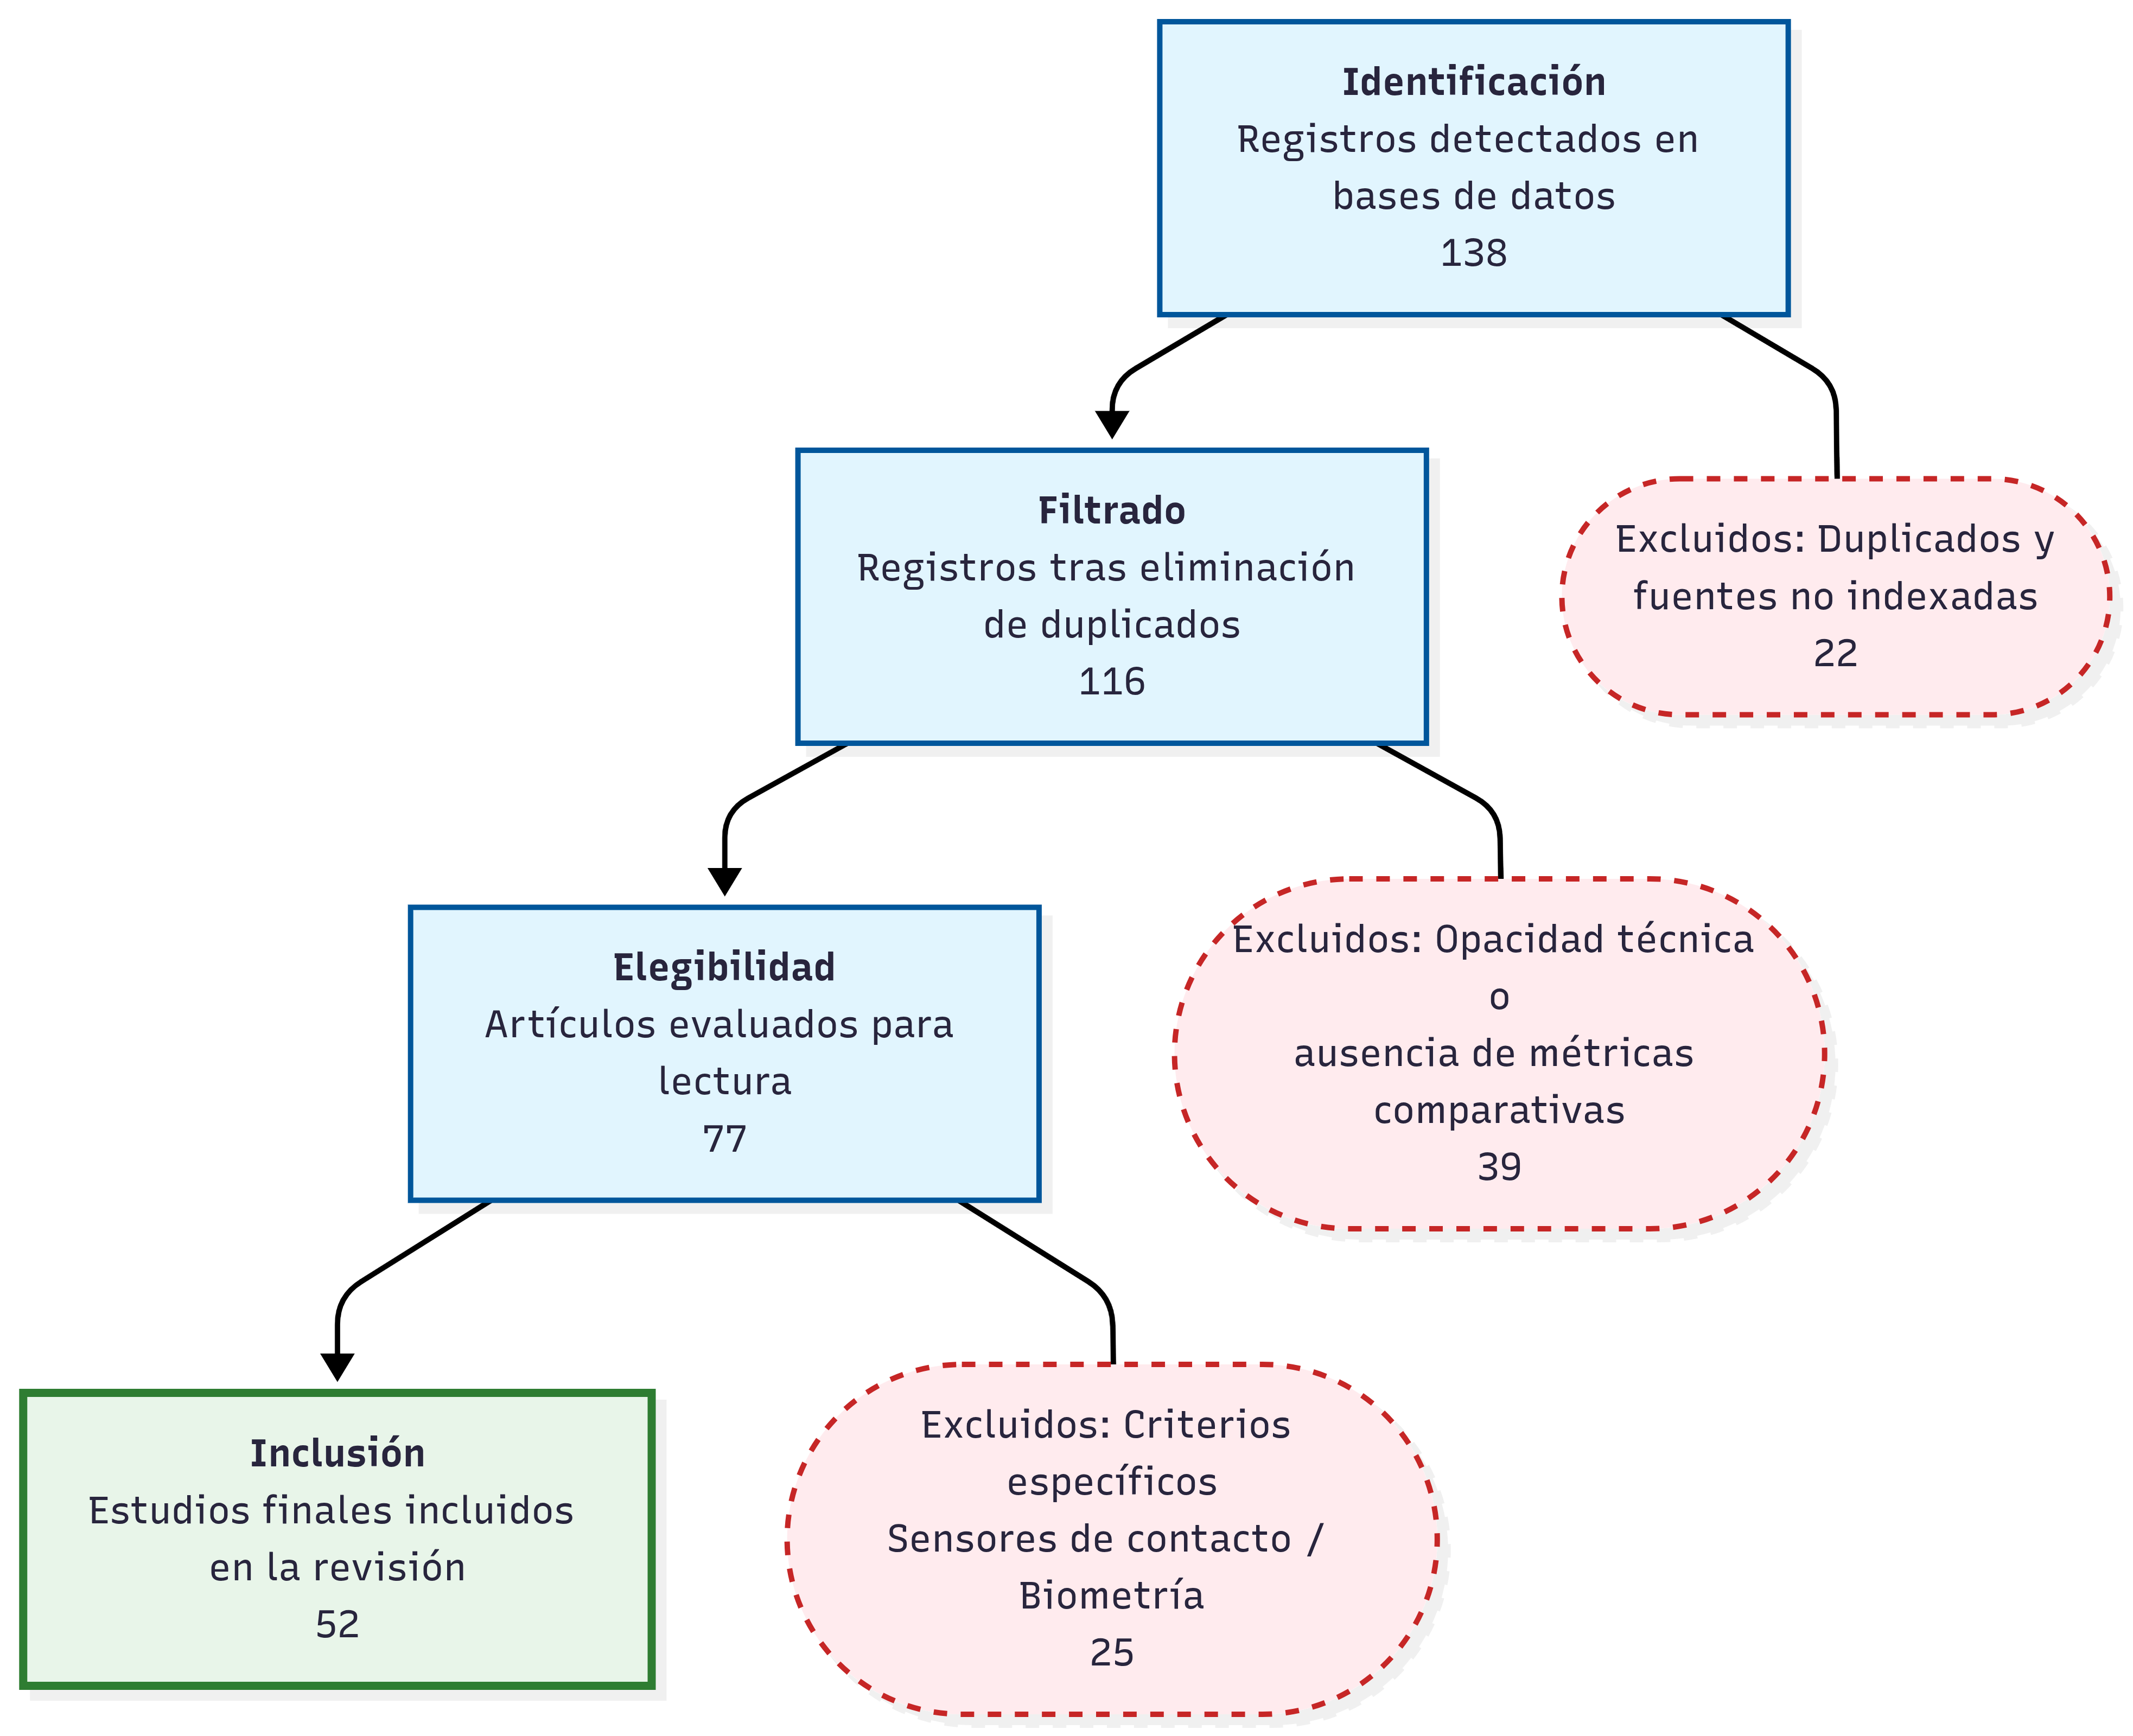
\includegraphics[scale=0.1]{images/DF_Filtros.png}
            \caption{Esquema PRISMA de selección de artículos.} 
            \label{fig:Flow}
        \end{figure}
\end{center}

\newpage
Complementariamente, se incluye un diagrama de Sankey (Flujo de Sankey de selección de artículos \ref{fig:Sankey}) con el fin de visualizar de manera proporcional la transición del corpus bibliográfico. 
A diferencia del diagrama de flujo tradicional, esta representación permite observar la magnitud de los descartes y, fundamentalmente, la distribución 
equilibrada de los 52 documentos finales a través de los cuatro pilares estratégicos de la investigación:

\begin{center}
\begin{figure}[h]

            \centering
            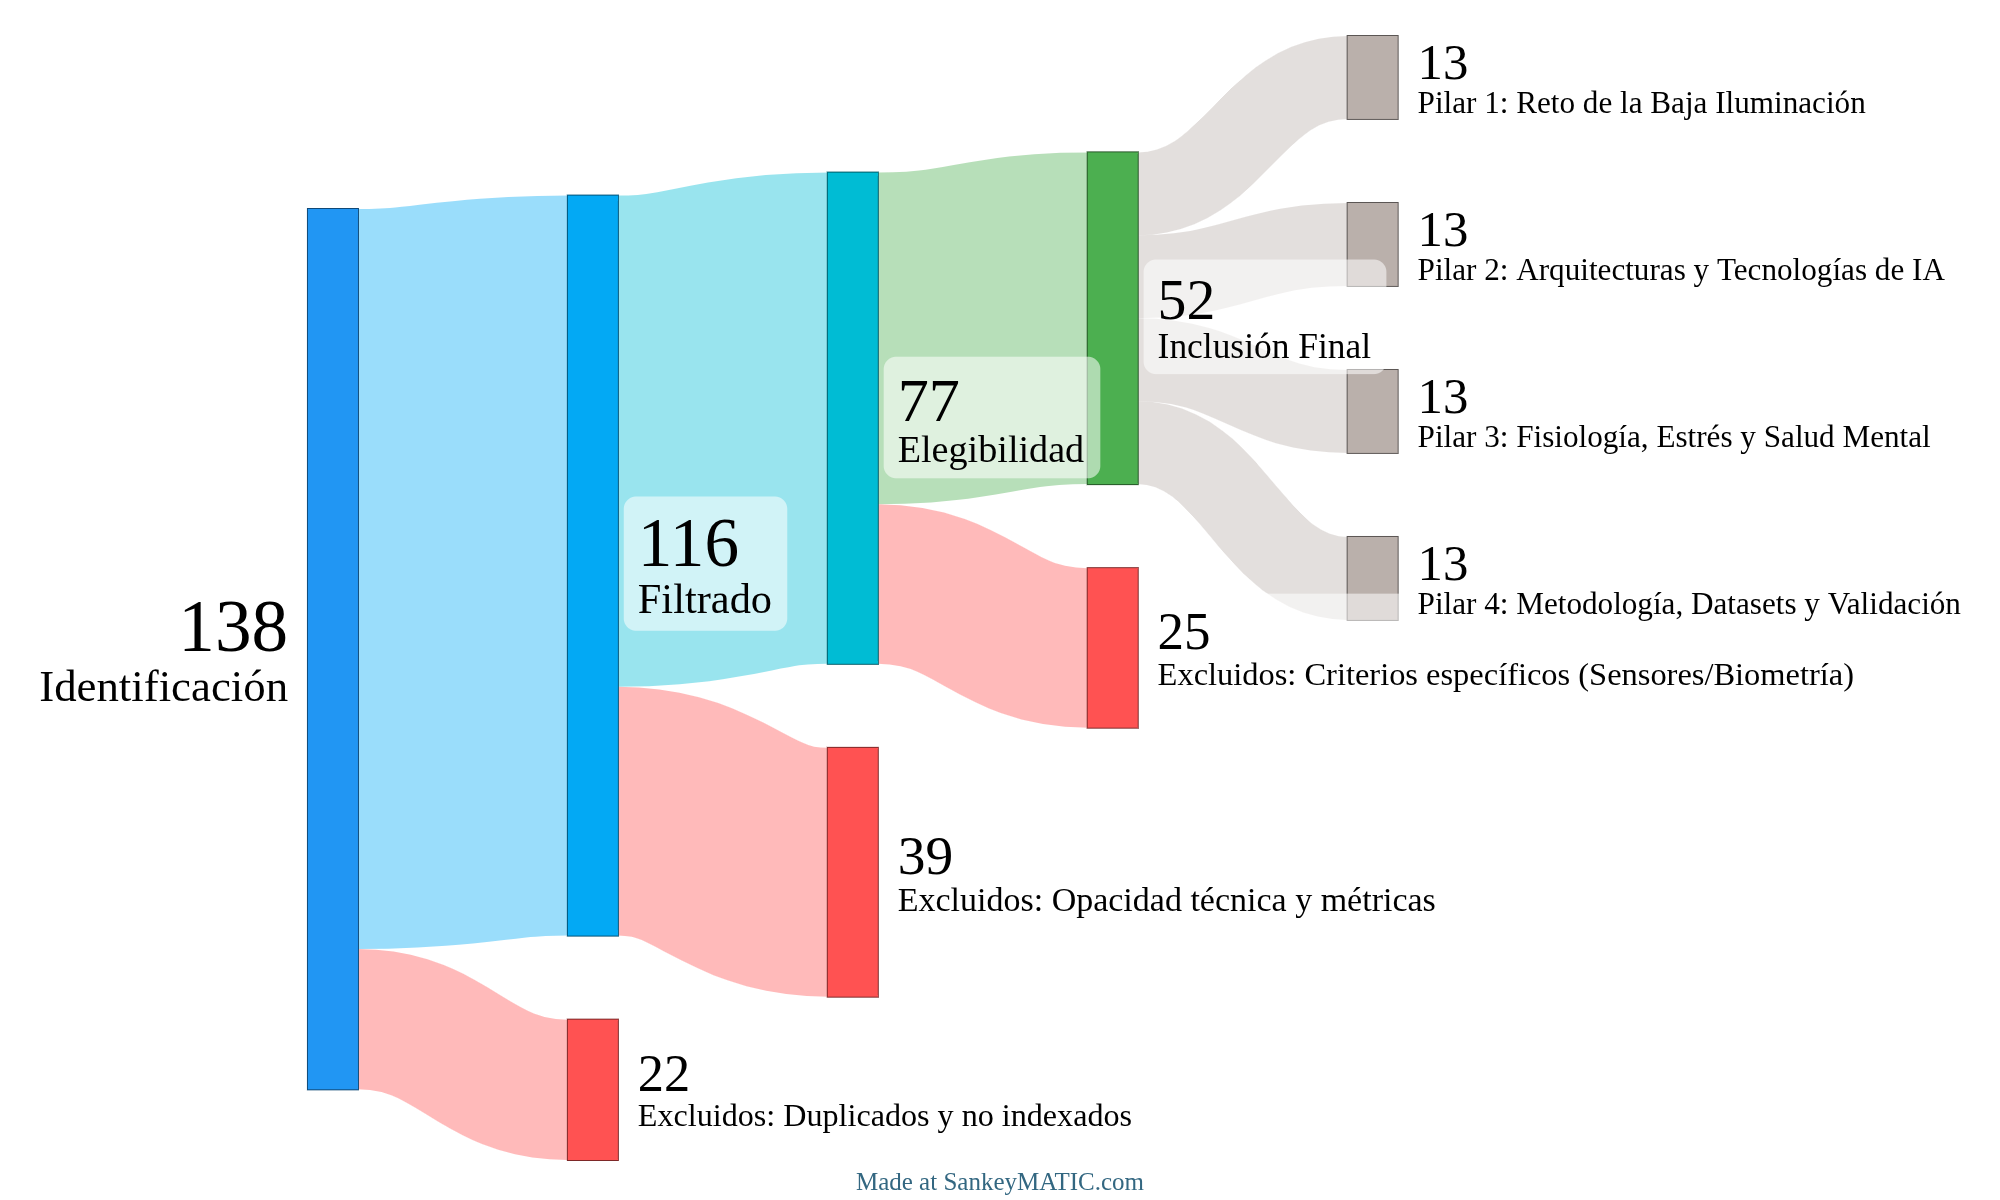
\includegraphics[scale=0.22]{images/SankeyFiltros.png}
            \caption{Flujo de Sankey de selección de artículos.} 
            \label{fig:Sankey}
        \end{figure}
\end{center}

De este modo, se procede al análisis sistemático de los 52 artículos seleccionados, los cuales constituyen la base para la consolidación del estado del arte. 
Este proceso se orienta a la identificación de brechas tecnológicas y hallazgos convergentes que permitan fundamentar la propuesta de investigación, asegurando 
una síntesis crítica que nutra la matriz de variables y la posterior fase experimental.

\newpage
\subsection{Distribución de los estudios}
De los 52 artículos científicos seleccionados para esta revisión, las plataformas IEEE Xplore y ScienceDirect (Elsevier) son las fuentes con mayor representación, 
sumando un total de 29 documentos que equivalen al 55.8\% del corpus bibliográfico. Esta concentración es consistente con la naturaleza técnica del proyecto, 
dado que estas bases de datos indexan las principales revistas de procesamiento de señales de video y arquitecturas de aprendizaje profundo. En la tabla (\ref{tab:distribucion_fuentes}) 
se puede apreciar las distribución de forma ordenada.

\begin{table}[htbp]
    \centering
    \caption{Distribución de artículos seleccionados por base de datos o fuente.}
    \label{tab:distribucion_fuentes}
    \begin{tabular}{|l|c|}
        \hline
        \textbf{Base de Datos / Fuente} & \textbf{Cantidad de Artículos} \\ \hline
        IEEE Xplore (Ingenierías)       & 15                             \\ \hline
        ScienceDirect (Elsevier)        & 14                             \\ \hline
        MDPI (Sensors / Electronics)    & 10                             \\ \hline
        arXiv (Literatura de frontera)  & 8                              \\ \hline
        Otras fuentes (Nature / PubMed) & 5                              \\ \hline
        \textbf{Total}                  & \textbf{52}                    \\ \hline
    \end{tabular}
\end{table}

Los estudios seleccionados presentan una ventana de publicación concentrada principalmente entre 2022 y 2026, asegurando que el análisis de los modelos Vision 
Transformers (ViT) y las arquitecturas Mamba representen el estado del arte más reciente en la detección de estrés mediante rPPG.

\subsection{Distribución temporal y por arquitectura}

Los estudios seleccionados para esta revisión presentan una ventana de publicación entre los años 2022 y 2026, con una tendencia creciente a partir del año 2024. 
Este incremento representa el 73\% del total de la muestra, lo que evidencia el auge actual de los modelos basados en atención global y su aplicación en la 
robustez de señales rPPG. El año 2024 destaca como el punto de mayor producción bibliográfica con 19 publicaciones, seguido muy de cerca por el año 2025 con 15 
estudios indexados. La tabla (\ref{tab:distribucion_anio}) representa la distribución de documentos por año.\\

\begin{table}[htbp]
    \centering
    \caption{Distribución de artículos seleccionados por año de publicación.}
    \label{tab:distribucion_anio}
    \begin{tabular}{|l|c|}
        \hline
        \textbf{Año de publicación} & \textbf{Cantidad de Artículos} \\ \hline
        2022                        & 6                              \\ \hline
        2023                        & 8                              \\ \hline
        2024                        & 19                             \\ \hline
        2025                        & 15                             \\ \hline
        2026                        & 4                              \\ \hline
        \textbf{Total}              & \textbf{52}                    \\ \hline
    \end{tabular}
\end{table}

\newpage
En cuanto a la distribución por arquitectura de los 52 artículos seleccionados, un análisis detallado de sus estructuras internas revela una taxonomía más 
diversa que la categorización genérica tradicional. Las \textbf{Redes Convolucionales (CNN) puras} abarcan 10 publicaciones (19.2 \%). No obstante, para 
superar las limitaciones de las convoluciones aisladas, la literatura ha explorado diversas combinaciones híbridas: 8 estudios (15.4 \%) emplean 
\textbf{modelos híbridos de CNN con redes recurrentes (CNN + LSTM/GRU)} enfocados principalmente en el modelado temporal de variaciones fisiológicas, 10 
estudios (19.2 \%) corresponden a \textbf{CNNs optimizadas con módulos de atención integrada} (como TS-CAN y Peak Attention) y 5 publicaciones (9.6 \%) 
representan \textbf{modelos híbridos de CNN 3D con Vision Transformers (CNN 3D -- ViT)} como PhysFormer y TransPhys, los cuales anteponen un 
\textit{Stem} convolucional para estabilizar la extracción local de la piel. Por su parte, los \textbf{Vision Transformers (ViT) puros} representan 7 
investigaciones (13.5 \%). Finalmente, los modelos emergentes de \textbf{Espacio de Estados (Mamba / SSM)} y los 
\textbf{métodos tradicionales de filtrado óptico} abarcan 6 artículos cada uno (11.5 \% respectivamente). Esta caracterización detallada demuestra la evolución continua hacia arquitecturas 
compuestas y evidencia la diversidad de mecanismos disponibles para abordar la 
resiliencia en penumbra, los cuales serán analizados y contrastados en el primer 
objetivo específico para seleccionar el más adecuado al alcance de este proyecto. 
En la tabla (\ref{tab:distribucion_modelos}) se presenta el desglose detallado de esta distribución:

\begin{table}[htbp]
    \centering
    \caption{Distribución por arquitectura de Inteligencia Artificial.}
    \label{tab:distribucion_modelos}
    \begin{tabular}{|l|c|}
        \hline
        \textbf{Arquitectura / Enfoque} & \textbf{Cantidad de Artículos} \\ \hline
        Redes Convolucionales (CNN Puras)               & 10                             \\ \hline
        CNN + Módulos de Atención (sin Transformer)     & 10                             \\ \hline
        Híbridos CNN + RNN / LSTM / GRU                 & 8                              \\ \hline
        Vision Transformers (ViT Puros)                 & 7                              \\ \hline
        Modelos de Espacio de Estados (Mamba / SSM)     & 6                              \\ \hline
        Métodos Tradicionales / Filtros Ópticos         & 6                              \\ \hline
        Híbridos CNN 3D + Vision Transformer (ViT)      & 5                             \\ \hline
        \textbf{Total}                        & \textbf{52}                    \\ \hline
    \end{tabular}
\end{table}

\newpage
De igual forma la tabla (\ref{tab:distribucion_q}) representa la distribución de artículos por cuartil, que representa el impacto de las investigaciones en este campo:

\begin{table}[htbp]
    \centering
    \caption{Distribución de artículos por cuartil.}
    \label{tab:distribucion_q}
    \begin{tabular}{|l|c|}
        \hline
        \textbf{Clasificación / Cuartil} & \textbf{Cantidad de Artículos} \\ \hline
        Q1                               & 22                             \\ \hline
        Q2                               & 20                             \\ \hline
        Sin categoría / Pre-prints       & 10                             \\ \hline
        \textbf{Total}                   & \textbf{52}                    \\ \hline
    \end{tabular}
\end{table}

Por último se presenta la tabla (\ref{tab:distribucion_paises}), un indicador de la distribución de investigación en este campo por paises, con un claro liderzago
por parte investigadores de universidades de China

\begin{table}[htbp]
    \centering
    \caption{Procedencia geográfica de la literatura seleccionada.}
    \label{tab:distribucion_paises}
    \begin{tabular}{|l|c|}
        \hline
        \textbf{País de origen} & \textbf{Cantidad de Artículos} \\ \hline
        China / Finlandia       & 25                             \\ \hline
        Corea del Sur           & 11                             \\ \hline
        Estados Unidos          & 6                              \\ \hline
        Europa (Francia, otros) & 5                              \\ \hline
        Otros (India, etc.)     & 5                              \\ \hline
        \textbf{Total}          & \textbf{52}                    \\ \hline
    \end{tabular}
\end{table}

\newpage

% \subsection{Análisis comparativo de modelos}

% A fin de comprender de forma comparativa el rendimiento teórico en condiciones ideales y la aplicabilidad clínica en el mundo real, es necesario analizar 
% cómo las arquitecturas actuales que han trabajado bajo un enfoque de evaluación lumínico o de movimiento, se comportan ante la degradación severa de la señal. Mientras que los resultados en entornos controlados sugieren una resolución 
% casi completa del problema de extracción del pulso, el Cuadro (\ref{tab:comparativa_modelos}) expone las diferencias entre los modelos dominantes cuando se enfrentan 
% a variables críticas como la iluminación deficiente, el ruido electrónico del sensor y la pérdida de píxeles:

% \begin{table}[htbp] 
%     \centering 
%     \caption{Comparativa de robustez y degradación de arquitecturas ante escenarios de ruido e iluminación deficiente.} 
%     \label{tab:comparativa_modelos} 
%     \begin{tabular}{|p{2.5cm}|p{2.3cm}|p{3.2cm}|c|p{4.8cm}|} 
%         \hline 
%         \textbf{Arquitectura} & \textbf{Modelo} & \textbf{Dataset (Reto)} & \textbf{MAE} & \textbf{Referencia y Hallazgo} \\ \hline
%         \textbf{CNN (2D-CNN)} & DeepPhys & BH-rPPG \newline \small{(Luz Baja)} & 21.76 & Yang, Wang y otros (2022). Falla sistémica ante la oscuridad; señal confundida con ruido electrónico. \\ \hline
%         \textbf{CNN (TS-CNN)} & TS-CAN & NICU-NPS \newline \small{(Penumbra)} & 12.73 & Yang y otros (2024). Las convoluciones puras colapsan en entornos clínicos oscurecidos. \\ \hline
%         \textbf{CNN (3D-CNN)} & PhysNet & MMPD \newline \small{(Luz Variable)} & 4.81 & Luo, Xie y otros (2024). Mayor estabilidad frente al ruido general comparado con arquitecturas ViT. \\ \hline
%         \textbf{Híbrido (CNN 3D + ViT)} & PhysFormer & MMPD \newline \small{(Movimiento)} & 13.64 & Yu, Shen y otros (2022). El mecanismo de atención global pierde fiabilidad ante ruido incontrolado. \\ \hline
%         \textbf{CNN (2D + TSM)} & EfficientPhys & MMPD \newline \small{(Realista)} & 12.79 & Luo, Xie y otros (2024). Fracaso en escenarios complejos frente a la robustez de las CNN. \\ \hline
%         \textbf{CNN (3D Contrastivo)} & ContrastPhys & COHFACE \newline \small{(Ruido Espacial)} & 10.10 & Nguyen, Bordallo y otros (2024). Fragilidad estructural ante la degradación artificial de píxeles. \\ \hline
%     \end{tabular}
% \end{table}

% %ModificadoSep2026
% Al analizar los resultados de la tabla (\ref{tab:comparativa_modelos}), se evidencia que las arquitecturas convolucionales puras sufren una degradación 
% severa en escenarios de baja iluminación. Modelos como DeepPhys registran un error de hasta 21.76 bpm en condiciones de penumbra debido a que la falta de 
% fotones confunde los filtros locales con el ruido térmico del sensor. Por su parte, aunque modelos como PhysNet muestran mayor estabilidad en iluminación 
% variable (MAE de 4.81 bpm), las convoluciones aisladas colapsan al intentar modelar dependencias espacio-temporales de largo alcance en entornos clínicos u 
% oscurecidos, como lo demuestra el desempeño de TS-CAN (MAE de 12.73 bpm).

% Por otro lado, los mecanismos de atención espacio-temporal y las arquitecturas híbridas no quedan exentas de vulnerabilidades. Como se observa en 
% PhysFormer (MAE de 13.64 bpm bajo movimiento), la atención global tiende a desestabilizarse cuando las fluctuaciones de luz o el movimiento incontrolado 
% alteran la homogeneidad de los parches visuales, asignando pesos de atención a regiones ruidosas.

% Esta evidencia demuestra que las aproximaciones de un solo paradigma resultan insuficientes para operar fuera de condiciones ideales de laboratorio. La 
% degradación observada en ambos frentes valida técnicamente la propuesta de este trabajo: en lugar de elegir entre convolución o atención global, es 
% necesario desarrollar una \textbf{arquitectura profunda híbrida (CNN 3D -- Vision Transformer)} que combine la fortaleza de ambos enfoques.

% \vspace{1em}

% La literatura sustenta esta integración híbrida a partir de dos factores metodológicos complementarios:

% \begin{itemize}
%     \item \textbf{Aporte del Stem Convolucional 3D (Sesgo Inductivo Espacial):} La inclusión de capas convolucionales 3D iniciales aporta el \textit{Inductive Bias} necesario para extraer características cromáticas locales de la piel de forma robusta, estabilizando la señal inicial y evitando que el ruido de baja iluminación corrompa la entrada del modelo.
%     \item \textbf{Aporte del Vision Transformer (Filtrado y Atención Temporal):} La integración posterior del módulo ViT permite modelar la periodicidad del pulso a largo plazo y filtrar de manera inteligente las sombras y variaciones globales del entorno que las convoluciones locales no logran abstraer.
% \end{itemize}

% De este modo, el trabajo conjunto entre el sesgo inductivo local de las CNNs 3D y el modelado contextual de los Vision Transformers se consolida como la solución adecuada para preservar la relación señal-ruido (SNR) y sostener la fiabilidad en la clasificación del estrés psicofisiológico bajo escenarios de penumbra.

% \subsection{Análisis Crítico de Arquitecturas Convencionales y la posibilidad de un Modelo Híbrido}

% En la literatura reciente, la arquitectura de fotopletismografía remota (rPPG) han sido empleadas en gran parte las Redes neuronales convolucionales para la extracción 
% conjunta de características espaciales y temporales a partir de secuencias de video facial \cite{yu2023physformer, cao2024stphys}. Sin embargo, estos
% autores también coinciden en que los núcleos convolucionales 3D poseen un campo receptor espacio-temporal propiamente limitado por su diseño local \cite{yu2023physformer, cao2024stphys}.

% En consecuencia se dificulta la captura de dependencias temporales de largo alcance, las cuales son 
% fundamentales para modelar la periodicidad de señales fisiológicas complejas, extraer métricas de variabilidad de la frecuencia cardíaca (HRV) y 
% discriminar estados psicofisiológicos como el estrés en secuencias extensas \cite{yu2023physformer, yu2024rgbnir}.

% A pesar de que los modelos que integran CNN y LSTM logran capturar secuencias extensas a través de la LSTM, fallan en el análisis de las relaciones 
% espaciales globales dentro del fotograma debido a la naturaleza local de las convoluciones de la CNN \cite{yu2023physformer}.

% Por otro lado, la introducción de arquitecturas basadas exclusivamente en Vision Transformers (ViT) ha permitido abordar la limitación del campo receptor 
% gracias al mecanismo de autoatención global, el cual conecta información entre fotogramas distantes en la secuencia \cite{yu2023physformer, yu2024rgbnir}.
% Sin embargo, advierten de igual manera que los Transformers puros presentan inconvenientes metodológicos significativos cuando se aplican de forma aislada en 
% el dominio del rPPG y con datos inadecuados porque carece de unos sesgos inductivos propios de las CNNs \cite{yu2024rgbnir}.

% En mayor detalle, carecen del sesgo inductivo de localidad espacial (*spatial inductive bias*) que caracteriza a las CNNs, lo que dificulta que la red 
% aprenda de forma nativa la estructura geométrica del rostro y las relaciones entre píxeles vecinos de la piel \cite{yu2024rgbnir}.

% Si se añade el factor de baja iluminación, las características de extracción se ven mayormente afectadas, bajo atenuación lumínica extrema, la relación 
% señal-ruido (SNR) de los videos cae progresivamente y el ruido termina perdurando en la señal \cite{chen2024image_en, wu2026udarppg}. 
% En las arquitecturas 3D-CNN puras, la falta de luz y la dispersión del ruido en las regiones locales provocan que los filtros convolucionales amplifiquen 
% el ruido del sensor, distorsionando la señal fisiológica \cite{cao2024stphys, wu2026udarppg}. Por su parte, en los Transformers puros, la ausencia de un 
% filtrado espacial previo hace que la autoatención global calcule relaciones directamente sobre *tokens* de parches oscuros y ruidosos, corrompiendo los 
% mapas de atención y propagando el error en las representaciones temporales \cite{chen2024image_en, wu2026udarppg, yu2023physformer}.

% La investigación reciente ha estado evaluando la combinación híbrida de bloques convolucionales 3D y capas de autoatención espacio-temporal y constituye 
% una alternativa técnica viable y equilibrada para mitigar las deficiencias individuales de ambos esquemas \cite{liu2023rppgmae, transphys2023}.

% \subsection{Representación de niveles de iluminación}

% De acuerdo con la Teoría Retinex \cite{chen2024image_en}, y el modelo de reflexión dicromática de la piel [\cite{camerabased2024wang}, \cite{chen2024image_en}],
% la intensidad de cada píxel en un fotograma $I(x,y)$ es el producto entre la reflectancia de la piel $R(x,y)$ (que contiene la variación de pulso rPPG) y 
% la mapa de iluminancia ambiental $L(x,y)$:\\
% $$I(x,y) = R(x,y) \cdot L(x,y)$$\\
% Esto indica que puede someterse a una degradación lumínica simulada dado que los sensores ópticos de las cámaras RGB operan con una respuesta lineal a la 
% luz en condiciones sin saturación. La degradación de cada pixel $I(x,y)$ puede simular niveles de iluminación dado que trabajan bajo control digital de intensidad de brillo de pixeles,
% simulando ruido de forma controlada. Existen datasets que controlan este ruido de forma física alterando la iluminación en niveles Lux de una fuente física, donde para otros escenarios
% puede ser controlada digitalmente.
% La siguiente tabla \ref{tab:comparativa_lux} contiene una comparación de Lux especifica y los estados de iluminación ambiental:

% \begin{table}[htbp] 
%     \centering 
%     \caption{Valores de Lux e iluminación ambiental} 
%     \label{tab:comparativa_lux} 
%     \begin{tabular}{|p{3cm}|p{3cm}|p{8cm}|} 
%         \hline 
%         \textbf{Condición de Iluminación} & \textbf{Iluminancia Física Medida (Lux)} & \textbf{Estado de la Señal rPPG en la Literatura} \\ \hline
%         \textbf{Alta} & 104.0 LUX \cite{chen2024image_en, yang2022assessment_dl} & Señal rPPG óptima, relación señal-ruido (SNR) alta \cite{yang2022assessment_dl} \\ \hline
%         \textbf{Media} & 42.4 LUX & Disminución moderada de la SNR, la cara se mantiene visible \cite{yang2022assessment_dl} \\ \hline
%         \textbf{Baja} & 8.0 LUX & Caída severa de la amplitud del pulso, el ruido de cuantización domina  \cite{yang2022assessment_dl} \\ \hline
%         \textbf{Extrema} & 1.0 a 4.0 LUX & Pérdida casi total del rostro y falla del seguimiento \cite{yang2022assessment_dl} \\ \hline
%     \end{tabular}
% \end{table}

% Como se aprecia en la anterior tabla \ref{tab:comparativa_lux}, la alta iluminación corresponde a un entorno controlado de estudio o laboratorio 
% ampliamente iluminado. Bajo estas condiciones, la cantidad de fotones que se reflejan en la microcirculación del rostro es óptima \cite{yang2022assessment_dl}.
% Esto genera una alta relación señal-ruido (SNR), permitiendo que las variaciones cromáticas asociadas al volumen de pulso sanguíneo (BVP) sean claramente 
% detectables por los sensores de la cámara \cite{yang2022assessment_dl}. Con respecto a las iluminaciones medias y bajas, de acuerdo con el modelo de 
% reflexión óptica de la piel, al reducirse drásticamente la iluminancia incidente ($L$), la luz reflejada difusa que transporta la información de la 
% pulsación arterial decae significativamente \cite{chen2024image_en}. Bajo este nivel de luxes, la pequeña variación pulsátil es eclipsada por el ruido de 
% cuantización del sensor fotográfico (ruido térmico y electrónico de la cámara), provocando que los algoritmos convencionales pierdan la capacidad de 
% rastrear la onda rPPG \cite{chen2024image_en, xi2022weighted}, lo que supone un reto para la extracción de la información de los modelos
% aplicados y futuramente desarrollados.



\subsection{Brechas identificadas}
El análisis del corpus bibliográfico revela algunas brechas relevantes que representan retos pero así mismo oportunidades para la investigación:

\begin{itemize}
    \item \textbf{Desconexión entre robustez en la estimación del pulso y fiabilidad del diagnóstico de estrés:} Existen múltiples arquitecturas diseñadas 
    específicamente para mitigar el efecto de la baja iluminación en la extracción del pulso (HR), como DeepPhys, PhysNet, PhysFormer y ST-Phys, entre otras. 
    Sin embargo, ninguna reporta el impacto de esta degradación sobre la Variabilidad de la Frecuencia Cardíaca (HRV) ni sobre tareas de clasificación 
    clínica del estrés, solo en el ritmo cardiaco. Se desconoce en qué punto un modelo robusto en la estimación de HR deja de sostener un diagnóstico confiable de estrés 
    \cite{chatzaki2025overview, morales2022towards, rodriguez2025datasets, acharya2025reliability, rodrigues2025evaluating, zhan2026hrv_long}.
    \item \textbf{Uso de videos oscurecidos por software:} Como casi no existen videos de personas grabadas en la oscuridad total, los investigadores sugieren 
    oscurecer los videos normales usando programas. Todavía falta comprobar si este método de oscurecer videos artificialmente afecta de la misma manera a todos 
    los tipos de modelos de IA \cite{nguyen2024artifact_resilience, ma2025rfbayes, liu2025synrppg, benezeth2024video, liu2023rppgmae}.
    \item \textbf{Falta de comparación bajo un protocolo clínico unificado:} 
    Aunque existen múltiples estrategias específicas redes convolucionales puras, híbridas CNN-ViT, modelos de espacio de estados para mitigar el ruido 
    lumínico, cada una ha sido validada en datasets distintos y bajo condiciones de degradación diversas (iluminación física vs. digital, distintos 
    niveles de atenuación). Esto impide determinar, bajo un mismo protocolo clínico como UBFC-Phys y su protocolo TSST, cuál preserva mejor la fiabilidad 
    del diagnóstico de estrés. \cite{transphys2023, effective2023cross, nguyen2024artifact_resilience, dehnad2024factorize, yu2023physformer, chang2025physvim, yan2025physmamba}.
\end{itemize}


\subsection{Hallazgos identificados}
Así mismo se revelan algunos hallazgos relevantes que acompañan el proceso de investigación. Su identificación es crucial y se definen posibles rutas en un mapa de trabajo investigativo:

\begin{itemize}
    \item \textbf{Fallas en los filtros de imagen:} Los filtros para aclarar videos (como el ajuste de brillo o contraste) crean distorsiones de color que dañan 
    la señal del pulso. Por esto, la capacidad de ver en la oscuridad debe ser una característica interna de la IA, y no depender de arreglos previos en el 
    video \cite{yang2022assessment_dl, yang2022image_en, xi2022weighted}.
    \item \textbf{Uso de una base de datos estándar:} La base de datos \textit{UBFC-Phys} es la más recomendada para este estudio. Al usar una prueba estándar 
    (TSST) para estresar a las personas, ayuda a que el movimiento del cuerpo no afecte los datos finales y los resultados sean más 
    reales \cite{chatzaki2025overview, sabour2023ubfcphys, rodriguez2025datasets}.
    \item \textbf{Punto de comparación (Línea base):} Con buena luz, los modelos de IA clásicos logran una precisión mayor al 85\% usando los datos del 
    corazón \cite{mouadili2025advancing, fontes2024enhancing, bahameish2024strategies}.
    \item \textbf{Mecanismos de extracción y focalización de características:} Se evidenció que los enfoques convolucionales emplean con frecuencia módulos 
    de diferenciación temporal (como la diferencia de fotogramas adyacentes) para suprimir la luminancia estacionaria y aislar las variaciones cromáticas 
    subyacentes. Por su parte, la integración de mecanismos de atención tanto en redes convolucionales como en modelos basados en Transformers permite 
    ponderar dinámicamente las regiones faciales con mayor perfused vascular (como mejillas y frente), optimizando la selección de la región de interés 
    (ROI) y mitigando el impacto del ruido ambiental en la señal fisiológica \cite{dehnad2024factorize, xue2025noncontact, zhao2024masked, cho2025dualbranch}.
\end{itemize}